% !TEX root = ../Ausarbeitung.tex
\section{Containertechnologien} 
\label{sec:Containertechnologien}

Im Laufe der  Containertechnologie traten verschiedene Implementierungen derselben auf. Hierbei waren die ersten Umsetzungen noch sehr einfach aufgebaut und wurden mit den Anforderungen an die Containerdienste immer komplexer. Im Folgenden findet sich eine Übersicht über die wichtigsten Technologien in der Containerisierung.

\begin{figure}[H]
	\begin{center}
		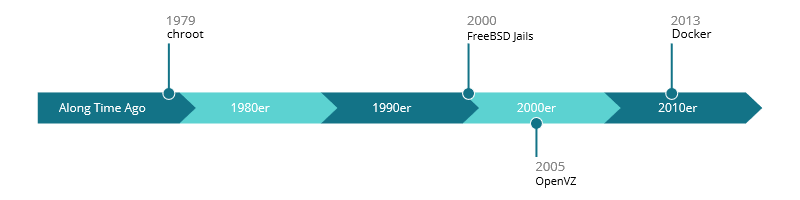
\includegraphics[width=0.8\textwidth]{ZeitContainer.png}
	\end{center}
	\caption[Containertechnologie im Laufe der Zeit]{Containertechnologie im Laufe der Zeit}
	\label{fig:CTZeit}
\end{figure}


\subsection{chroot}
\label{sec:chroot}

Chroot ist ein Befehl, der schon früh in Unix-Systemen eingebaut wurde. Er ermöglicht es einem Prozess ein andres Rootverzeichnis zu geben. Wird in einem Programm \code{chroot()} aufgerufen wechselt es das Verzeichnis und kann nicht auf Dateien außerhalb der zugewiesenen Struktur zugreifen. Diese Abschottung eines Prozess war nie als Sicherheitsfeature vorgesehen und wird hauptsächlich zur Virtualisierung eingesetzt. Mit dem Befehl können einzelne Prozess auf Dateiebene von anderen Anwendungen getrennt werden, weitere Sicherheitsmechanismen oder Isolierungen gibt es nicht.\cite{IEEE7830207,569694, MANPAGE01}

\subsection{OpenVZ}
\label{sec:OpenVZ}


\subsection{LXC}
\label{sec:lxc}



\subsection{LXD}
\label{sec:lxd}


\subsection{Windows Containers}
\label{sec:WindowsContainers}

\subsection{Docker}
\label{sec:Docker}

\subsection{Mesos}
\label{sec:Mesos}

\subsection{rkt}
\label{sec:rkt}

\subsection{FreeBSD jails}
\label{sec:jails}

